\section {Descripción y módulos del sistema}
% \section{¿Para qué sirve el sistema?}

  \subsection{Arquitectura general}
    \paragraph{Para desarrollar un sistema de recomendacion se han planteado los siguientes módulos funcionales de la API, el cual será utilizado por el desarrollador final para que, en conjunto con su aplicación final realice la integración de las funciones disponibles en el API junto al sistema de recomendación final. Esto se puede denotar en el siguiente diagrama.}

\newpage
    \begin{landscape}
      \begin{figure}[h!]
      \centering
      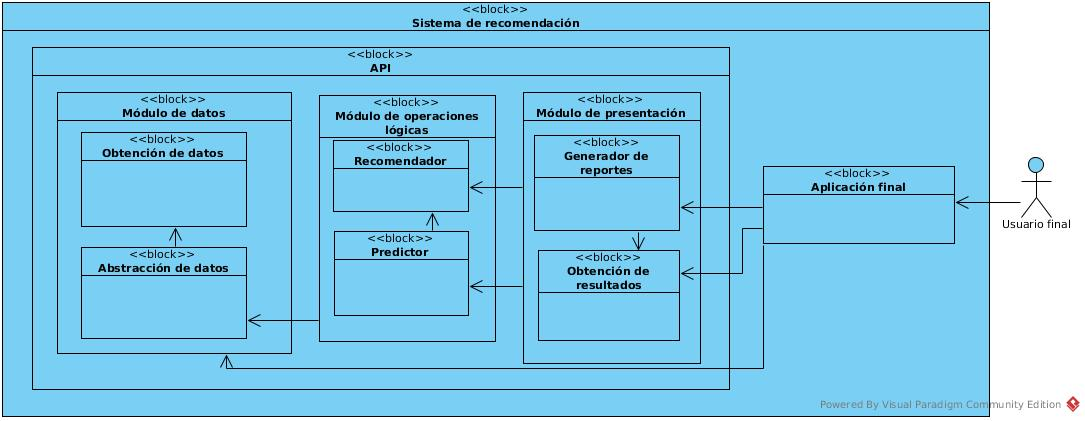
\includegraphics[width=22.5cm,height=12cm]{./images/architecture_diagram.jpg}
      \caption{Diagrama general del sistema}
    \end{figure}
    \end{landscape}
  \newpage

\paragraph{Cómo se apreciar en el diagrama, el sistema se encuentra dividido en tres módulos básicos además de la aplicación final que hace uso de los módulos de la API.}
    \begin{itemize}
    \item Módulo de datos
    \item Módulo de operaciones lógicas
    \item Módulo de presentación
    \item Caso de estudio ó aplicación final
  \end{itemize}

\subsection{Módulos de la API}
  \subsubsection{Módulo de abstracción de datos}
    \paragraph{Este módulo es el encargado de la obtención de datos para su adecuada manipulación dentro de los objetivos del sistema, es decir, permitirá el manejo de los datos estandarizandolos a un modelo de datos base que permitirá tener la funcionalidad del sistema de recomendación de manera adecuada. }
    \paragraph{Se presenta como un módulo conformado por diferentes interfaces de conexión para fuentes de datos, como pueden ser ficheros de texto o la conexión a un gestor de base de datos. Tiene una interacción directa con el módulo de operaciones lógicas dentro del sistema.}

  \subsubsection{Módulo de operaciones lógicas}
    \paragraph{El módulo de operaciones lógicas permitirá, haciendo uso de la información almacenada, obtener recomendaciones y predicciones de los diferentes artículos deacuerdo a diferentes clasificaciones con base en los principales tipos de recomendacion existentes: basados en contenido y colaborativos. Cabe destacar, la constante operación de este módulo para el aprendizaje y mejora constante de las recomendaciones.}

  \subsubsection{Módulo de presentación}
    \paragraph{Haciendo uso del módulo de operaciones lógicas, este módulo pretende brindar la funcionalidad de mostrar en forma de reportes tabulares, los resultados obtenidos de la recomendación al ser integrado en la aplicación final.}

\subsection{Aplicación final}
  \subsubsection{Definición}
    \paragraph{En este caso, la aplicación final hará uso de las funciones proporcionadas por los distintos módulos que conforman la API para obtener recomendaciones de los datos que pertenezcan a su caso de estudio. Interactúa directamente con el módulo de abstraccion de datos y con el módulo de presentación para hacer uso de la funcionalidad permitida por el API. En este caso, la aplicación final se verá reflejada en un sistema web que permita denotar la funcionalidad de la API para un conjunto de datos de platillos y restaurantes.}